% Machine Learning 
\section{Machine Learning}
\begin{frame}{What is Artificial Intelligence?}
    Artificial intelligence is the simulation of human intelligence processes by computer systems. These processes include \textbf{learning} (the acquisition of information and rules for using the information), \textbf{reasoning} (using rules to reach approximate or definite conclusions) and \textbf{self-correction}.

    \pause

    AI can be categorized as either \textbf{weak} or \textbf{strong}.

    \pause

    \begin{block}{Strong AI}
		Also known as artificial general intelligence. Is an AI system with generalized human cognitive abilities. When presented with an unfamiliar task, a strong AI system is able to find a solution without human intervention.
    \end{block}

    \pause

    \begin{block}{Weak AI}
		Also known as narrow AI. Is an AI system that is designed and trained for a particular task.
    \end{block}
\end{frame}

\begin{frame}{AI in perspective}
    \only<1>{
        \begin{figure}
            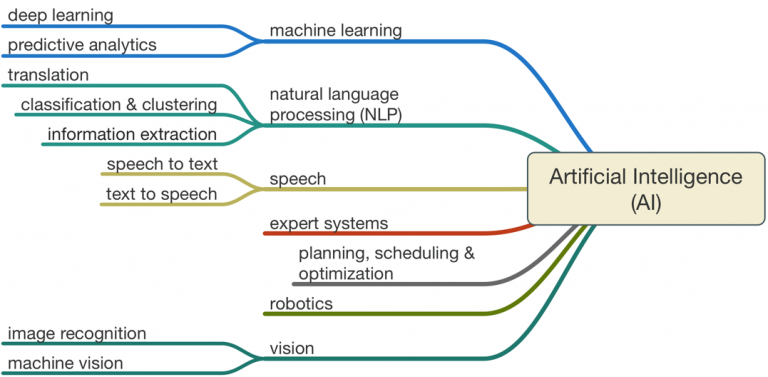
\includegraphics[width=\textwidth]{img/tree-ai.png}
        \end{figure}
    }

    \only<2>{
        \begin{figure}
            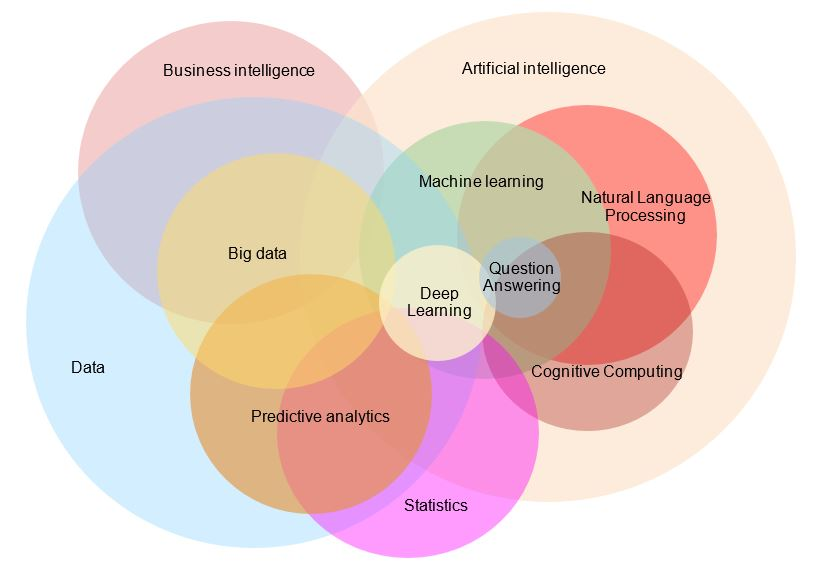
\includegraphics[width=\textwidth]{img/venn-ai.jpeg}
        \end{figure}
    }

    \only<3>{
        \begin{figure}
            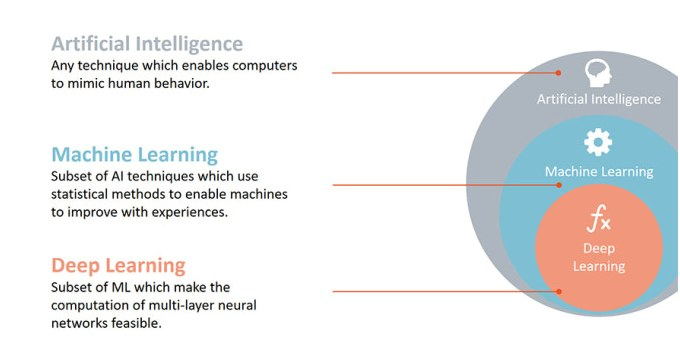
\includegraphics[width=\textwidth]{img/venn-ai-simplified.jpeg}
        \end{figure}
    }
\end{frame}

\begin{frame}{What is Machine Learning?}
    The science of getting a computer to act without programming. There are three types of machine learning algorithms:

    \pause

    \begin{block}{Supervised learning}
        Data sets are labeled so that patterns can be detected and used to label new data sets.
    \end{block}

    \pause

    \begin{block}{Unsupervised learning}
        Data sets aren't labeled and are sorted according to similarities or differences.
    \end{block}

    \pause

    \begin{block}{Reinforcement learning}
        Data sets aren't labeled but, after performing an action or several actions, the AI system is given feedback.
    \end{block}
\end{frame}

\begin{frame}{Supervised Learning}
    \begin{figure}
        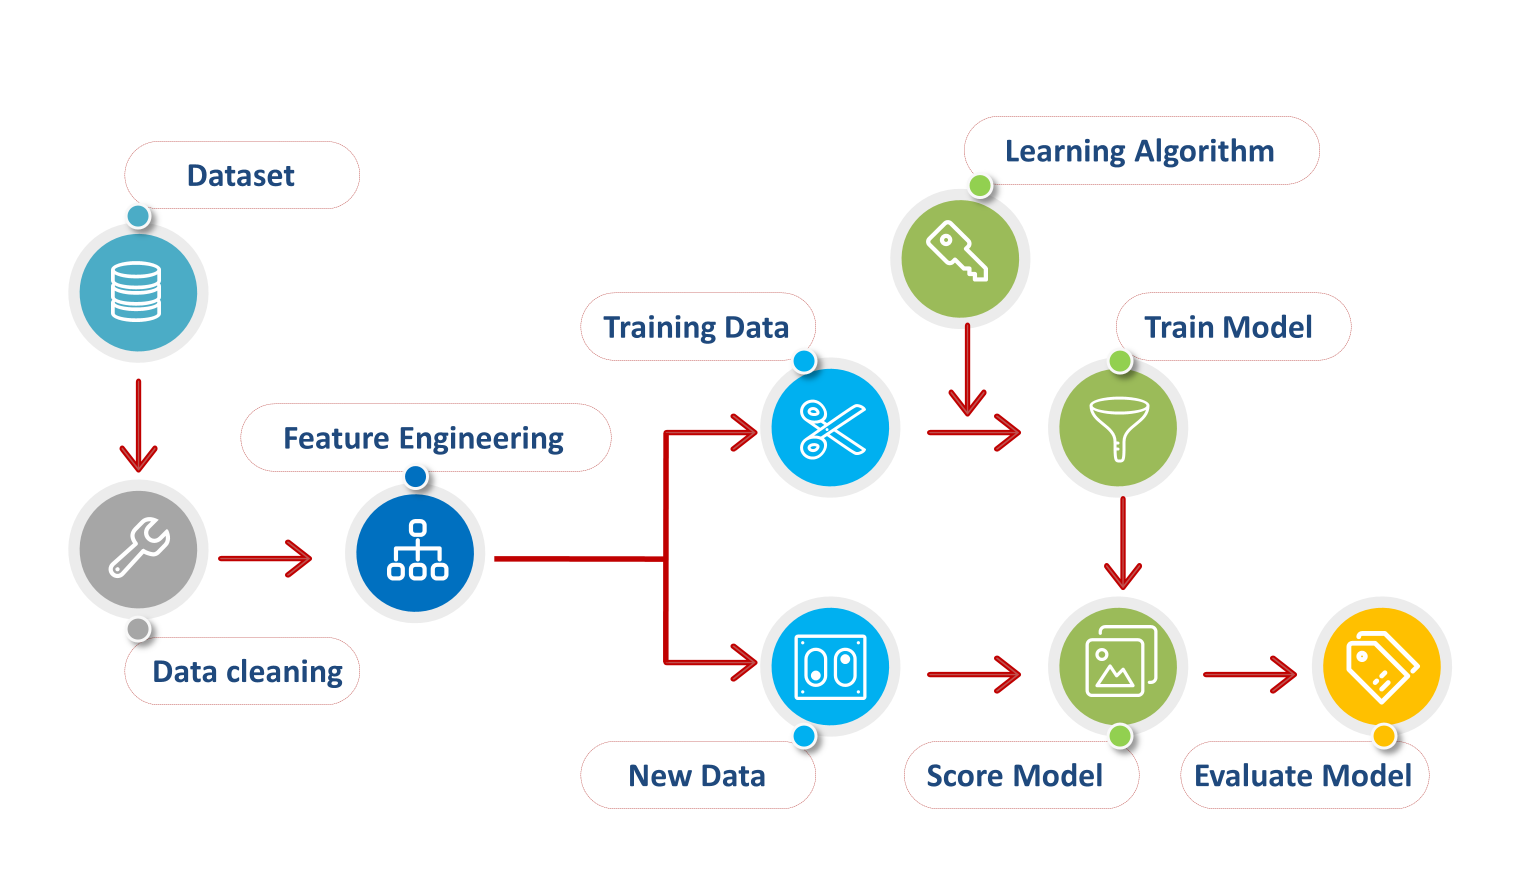
\includegraphics[width=\textwidth]{img/training-process.png}
    \end{figure}
\end{frame}

\begin{frame}{The Model}
    We are going to build a model that performs a sentiment analysis over a text and concludes if it is positive or negative.

    \textbf{Input:} A text (a list of integers representing each word).

    \textbf{Output:} 0 (negative) or 1 (positive).

    \begin{figure}
        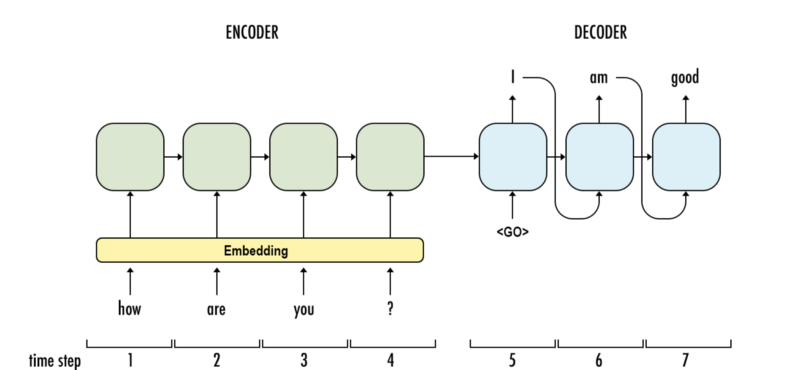
\includegraphics[width=\textwidth]{img/lstm-model.png}
    \end{figure}
\end{frame}

\begin{frame}{Training Dataset}
    The dataset used for training this model is based on movie's reviews from IMDB.

    \qquad

    \rowcolors{1}{}{gray!20}
    \begin{tabular}{lcc}
        \toprule
        \multicolumn{1}{c}{\textbf{Text input}} & \textbf{Input} & \textbf{Output} \\
        \midrule
        the as you with out themselves... & [1, 14, 22, 16, 43, 530, ...] & 1 \\
        the thought solid thought sena... & [1, 194, 1153, 194, 8255, ...] & 0 \\
        the as there in at by br of su... & [1, 14, 47, 8, 30, 31, 7, ...] & 0 \\
        the of bernadette mon they hal... & [1, 4, 18609, 16085, 33, ...] & 1 \\
        the sure themes br only acting... & [1, 249, 1323, 7, 61, 113, ...] & 0 \\
        \bottomrule
    \end{tabular}
\end{frame}
